\section[Náhodná procházka]{Náhodná procházka při simulaci životního cyklu neutronů v jaderném reaktoru}

Jak bylo zmíněno, ýpočty ve stochatických kódech probhají díky simulaci tzv. \textbf{random walks - náhodné procházky} dané částice, tedy simulace skutečného života dané částice. K tomu je potřeba znát pár základů.

\subsection{Matematická vsuvka}

\subsubsection{Generace pseudonáhodných čísel}

Jde o stochastickou/pravděpodobnostní metodu, tedy základem je generování náhodných čísel. Jelikož ke generaci dochází strojově, nebude nikdy možné stanovit skutečně náhodná čísla, pouze tzv. pseudonáhodná. O to větší problém je vytvořit sekvenci náhodných/pseudonáhodných čísel tak, aby se neopakovaly. K tomu se ve většině kódů využívá tzv. \textbf{linear congruential random numbers generator}:

$$ S_{i+1} = ( S_i \cdot g + c ) \: \text{mod} \: 2^m, $$

kde $S_i$ značí seed (typicky nějaké velké číslo, pokaždé jiné), $g$ značí generátor/násobič (opět veliké číslo, to může být stejné), $c$ značí přírůstek (může být 0, 1, nebo opět jakékoliv) a z toho všeho určíme modulus (tedy zbytek po dělení) nějakého čísla $2^m$.

Přesnou kombinací těchto čísel je možné stanovit konkrétní generátor, např. MCNP využívá: $m = 63$, $g$ je různé a $c = 1$.

\subsubsection{Random Sampling - Náhodné vzorkování}

Dále je potřeba navzorkovat daná čísla podle jistých pravděpodobnostních funkcí $f(x)$. Generátor náhodných čísel nám poskytne uniformní rozdělení na intervalu (0,1), nicméně např. k rozptylu dochází pod jistým úhlem s danou pravděpodobností, nebo energie vzniklých neutronů také mají jistou pravděpodobnost.

Máme-li tedy danou pravděpodobnostní funkci (PDF) $f(x)$ normovanou na 1. Z té jsme schopni určit distribuční funkci (CDF) $F(x)$ jako postupný integrál:

$$ F(x) = \int_{-\infty}^x f(y) \text{d}y. $$

Označíme-li uniformní náhodná čísla jako $\xi$, ale my chceme získat/navzorkovat hodnoty $x$, pak tedy hledáme relaci mezi:

$$ F(x) = \xi \iff x = F^{-1}(\xi). $$

To je možné určit:

\begin{itemize}
  \item \textbf{direct sampling - přímé vzorkování}, tedy napřímo. Není možné vždy, může být zdlouhavé a koplikované (jednoduché např. u konstanty).
  \item \textbf{rejection sampling - metoda odmítnutí}, mnohem více univerzálmí metoda.
\end{itemize}

Nejprve se stanoví konstanta $c \geq 1$ a další hraniční PDE $g(x)$ kterou je možné navzorkovat napřímo (např. konstanta) tak, aby pro všechna $x$ platilo:

$$ f(x) \leq c g(x). $$

Nejprve navzorkuji danou $\bar{x}$ z funkce $g(x)$ (to je jednoduché, udělám to napřímo). Dále naleznu nějakou hodnotu $\xi$  jednotkového intervalu (0,1), a pokud platí, že:

$$ \xi \leq \dfrac{f(\bar{x})}{c g(\bar{x})}, $$

pak mohu s jistotou říci, že zároveň $\bar{x}$ je navzorkována i z původní $f(x)$. Je to v podstatě stejný způsob, jako když se integrauje přes Monte-Carlo. Vybírám hodnoty z intervalu (0,$cg(x)$), a pokud platí, že hodnota je zároveň v intervalu (0,$f(x)$), tak ji vezmu, jinak ne, viz obrázek \ref{rejection}.

\begin{figure}[H]
  \centering
  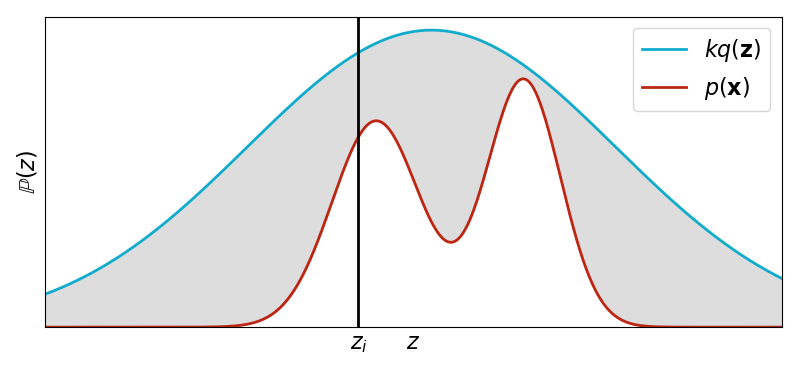
\includegraphics[width=0.7\textwidth]{img/rejection_sampling.png}
  \caption{Metoda odmítnutí.}
  \label{rejection}
\end{figure}

\subsection{Popis náhodné procházky}

Schematicky je náhodná procházka jednoduchá:

\begin{enumerate}
  \item[1.] Vznik -- částice nejprve vznikne, buď z externího zdroje, nebo za pomoci štěpení či (n,xn) reakce.
  \item[2.] Tracking -- částice se nějak pohybuje v daném prostředí. Sleduje se kudy prochází, jakými geometrickými hranicemi apod.
  \item[3.] Reakce -- tím, jak částice prochází prostředím, tak interaguje s okolní látkou, čímž se mění její směr, energie a v případě implicitní metody i váha
  \item[4.] Detektory/Tallies -- statistické vyhodnocení dané reakce.
  \item[5.] Zánik -- případné vyhodnocení za pomoci redukce variance.
\end{enumerate}

Toto se opakuje tisíckrát-milionkrát. 4ím větší geometrie, tím více částic je potřeba na detailnější prozkoumání celého systému. Na základě všech dat se poté vyhodnotí detektory, koeficient násobení, reakční rychlosti apod.

\subsubsection{Vznik}

Částice nejprve vznikne. Pokud máme externí zdroj, tak je dopředu nadefinováno energetické a směrové rozdělení. Pokud jde o zdroj ze štěpení, tak je třeba uvažovat energetické vzorkování přes štěpné spektrum a uniformní směrovou distribuci.

\subsubsection{Tracking}

Pokud znám počáteční energii a směr, je třeba určit, za jakou dobu dojde k další reakci (která se bude odehrávat na jiném místě). Opět se postupuje přes pravděpodobnostní PDE funkci ve tvaru:

$$ f(x) = \Sigma_\text{t} e^{-x \Sigma_\text{t}} $$

a distribuční CDF funkci:

$$ F(x) = 1 - e^{-x \Sigma_\text{t}}. $$

V tomto případě je CDF funkci možné vyjádřit pomocí přímého vzorkování jako:

$$ x = -\dfrac{1}{\Sigma_{\text{t}}} \text{ln}(1-\xi) = -\dfrac{1}{\Sigma_{\text{t}}} \text{ln}(\xi), $$

kde $\xi = F(x)$ navzorkujeme rovnoměrně z intervalu (0,1). 

Tohle platí, je-li geometrie složena homogenně pouze z jednoho materiálu. Máme-li ale geometrii s různými materiály (a tedy i různými $\Sigma_{t})$, je třeba postupovat postupně. Rozlišují se 2 přístupy:

\begin{itemize}
  \item Surface-tracking,
  \item Delta-tracking.
\end{itemize}

V případě \textbf{Surface-trackingu} se uplatňují izolované 2 výpočty před a za hranicí (tedy v materiálu 1 a 2). Má-li být zvdálenost mezi reakcemi $x$ delší, než je přímá trasa k hranici $d$ (tedy dojde-li k překročení hranice), musí se výpočet rozepsat, protože v novém materiálu už zbylé $x$ bude logicky jiné, kvůli jinému $\Sigma_\text{t}$. V novém materiálu tedy platí:

$$ e^{-x_2 \Sigma_2} = e^{-(x_1-d)\Sigma_2} $$

z čehož se vyjádří $x_2$ a pro celou dráhu $x$ bude platit:

$$ x = d + x_2 = d + (x_1 - d) \dfrac{\Sigma_1}{\Sigma_2}. $$

Opět, platí-li, že $x_2$ je opět větší než vzdálenost k další hranici, postupujeme pořád obdobně, dokud nevyjde, že $x_i$ skutečně skončí v daném materiálu. Hlavní filosofie tedy je, že se výpočet na každé hranici zastaví a podle aktuálního $\Sigma_\text{t}$ se přepočte vzdálenost mezi reakcemi $x$.

V případě \textbf{Delta-trackingu} se postupuje jinak, bez zastavování se na každé hranici. Cílem je stanovení virtuálního $\Sigma_0$, který by reprezentoval veškeré materiály nacházející se v daném směru, dle vztahu:

$$ \Sigma_0 = \Sigma_\text{m} - \Sigma_\text{t}, $$

kde $\Sigma_\text{m}$ značí maximální možný průřez, který se v systému vyskytuje (dává tedy horní odhad). Známe-li počáteční směr, určí se vzdálenost $x$ mezi reakcemi za pomocí pouze $\Sigma_\text{m}$ (tím získáme dolní odhad vzdálenosti), kde dojde k virtuální reakci. To, jestli dojde či nedojde k reakci, se určí dle pravděpodobnosti:

$$ P = \dfrac{\Sigma_0}{\Sigma_\text{m}} = 1 - \dfrac{\Sigma_\text{t}}{\Sigma_\text{m}}. $$

Pokud dojde k zamítnutí, proces pokračuje dál, dokud nedojde ke skutečné reakci. Výhody Delta-trackingu jsou patrné hlavně v momentu, kdy geometrie obsahuje spoustu ploch.

\subsubsection{Reakce}

Nyní jsme už v bodě, kde dojde k nějaké reakci, zbývá zjistit k jaké. To se opět určí pravděpodobnostně, tedy to, že dojde k $i$-reakci na $m$-izotopu určuje vztah:

$$ P = \dfrac{\Sigma_{i,m}}{\Sigma_\text{t}}. $$

V případě absorbce se dále může uplatnit redukce variance. V případě rozptylu se dále musí určit, pod jakým úhlem a s jakou energií se neutron rozptýlí. V případě štěpení kolik neutronů se emituje, atd. 

\subsubsection{Detektory}

V posledním případě zbývá zaznamenat dané reakce a určit nějakou integrální hodnotu. Může jít o hustotu toku, hustotu proudu, reakční rychlosti apod. Dá se postupovat analogově/implicitně, viz předešlá otázka.

Neméně důležité je zapracování nejistot. U výsledků se předpokládá Gaussovské rozdělení kolem nějaké střední hodnoty s daným rozptylem. Čím větší statistika, tím menší rozptyl. K tomuto určování se aplikují jakési matematicko-statistické nástroje, o kterých nemám ponětí, nicméně bavili jsme se o tzv. \textbf{Central Limit Theorem}, který tohleto umí dělat.

Výsledky jdou posléze i kombinovat mezi sebou. Dále se hodí vědět, že celkový rozptyl klesá s odmocninou celkové generace, tedy:

$$ \sigma^2 = \dfrac{\sigma^2_i}{N}. $$

\subsubsection{Zánik}

Nakonec neutron zanikne a už dále neexistuje :(